\subsection{Overview}
Given the nature of the application, a three layer approach has been chosen.\newline
\begin{figure}[h!]
	\centering
	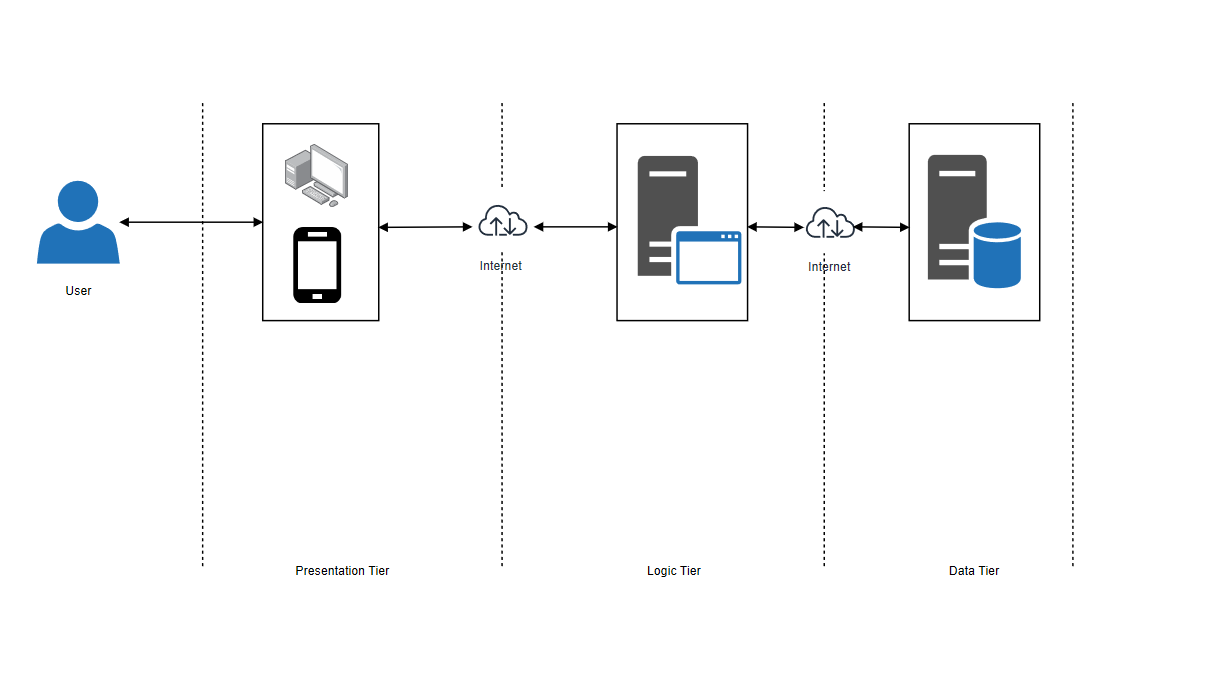
\includegraphics[width=\textwidth]{Images/three_layer}
	\caption{Three layer structure}
\end{figure}
\newline
As shown by the image above, the three layers consist in the presentation tier, the logic tier and the data tier
\begin{itemize}
\item Presentation Tier: consists of the user interfaces for all of the three clients (RegularUser, Policeman and MunicipalAuthority) and is used by the user to interact with both the application logic and Google Maps APIs \newline
\item Logic Tier: consists of the servers used to control the functionalities of the application, interacts with both the presentation and data tiers \newline
\item Data Tier: consists of the database server (where both user data and data generated by the application are stored), interacts only with the logic tier \newline
\end{itemize}
\newpage
\subsection{Component view}
\subsubsection{Introduction}
The following diagram represents the interface structure of the system, focusing on the application server structure. \newline
\begin{figure}[h!]
	\centering
	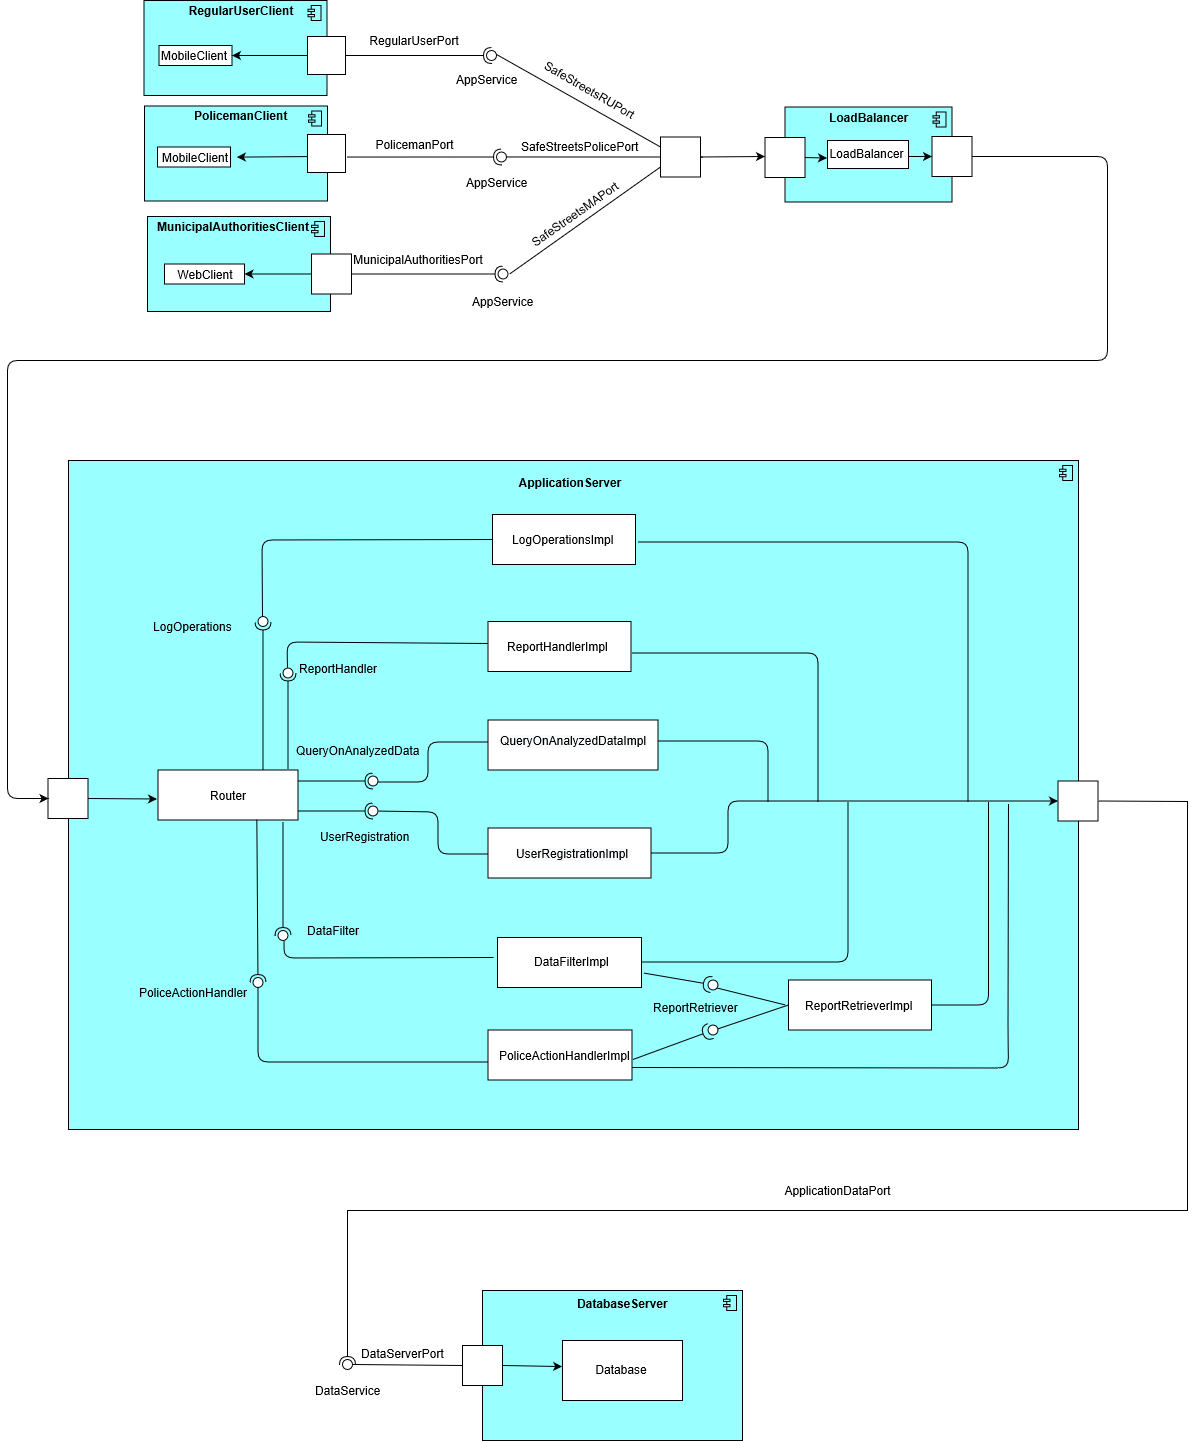
\includegraphics[width=\textwidth]{Images/component_diagram_beta}
	\caption{Component diagram}
\end{figure}

As shown above, the application logic is stored on the application server, while the clients just contain what is mandatory in order to contact the application server and to carry on basic operations  (thin client).\\
\subsubsection{Server}
We will now proceed to give a brief summary of the role of the components listed above:
\begin{itemize}
\item QueryOnAnalizedData: allows the RegularUser profiles to access data about the reports in a certain area or other information already analized by the MunicipalAuthorities
\item PoliceActionHandler: allows the policemen to take action on user made reports or to compile reports themself. The actions performed by the police consist in compiling reports (of which they will take care right away), marking themselves as dispatched towards a report, mark a report as wrong or signal that a traffic ticket has been written as a consequence of a reported traffic violation
\item ReportRetriever: this component is used by PoliceActionHandler and DataFilter in order to retrieve all the reports regarding the same violation (not just violation type, but also time, plate and location) as a given one. 
\item ReportHandler: this component manages users' submissions of reports about traffic violations. The reports are analyzed, authenticated and then strored inside the application DB
\item UserRegistration: this component allows the registration of all types of users. Note that, while RegularUser profiles registration is done by the user themselves, Authority profiles (Policeman and MunicipalAuthority) can only be registered by a system admin
\item LogOperations: this component takes care of the login and logout operations for all types of User profiles
\item DataFilter: allows MunicipalAuthority profiles to perform data-mining activities,  as well as cross-analyze external information (such as data about crashes in an area provided by a municipality ) with user-submitted reports
\end{itemize}
The logic of the application works based on the afromentioned components: they grant all the functionality needed to satisfy the system's goals (for a more in-depth analysis see chapter 4).
In the next two pictures more information about the system will be provided: the first represents a more accurate version of the class diagram presented in the RASD; the second includes a schema of the relationship between the classes interfaces and implementations of said interfaces. \newline
Note that, when compared to the class diagram present in the RASD, the class Photo is missing: this is so because of the Base64 encoding for the photos that has been chosen to represent them inside reports.

\begin{figure}[H]
	\centering
	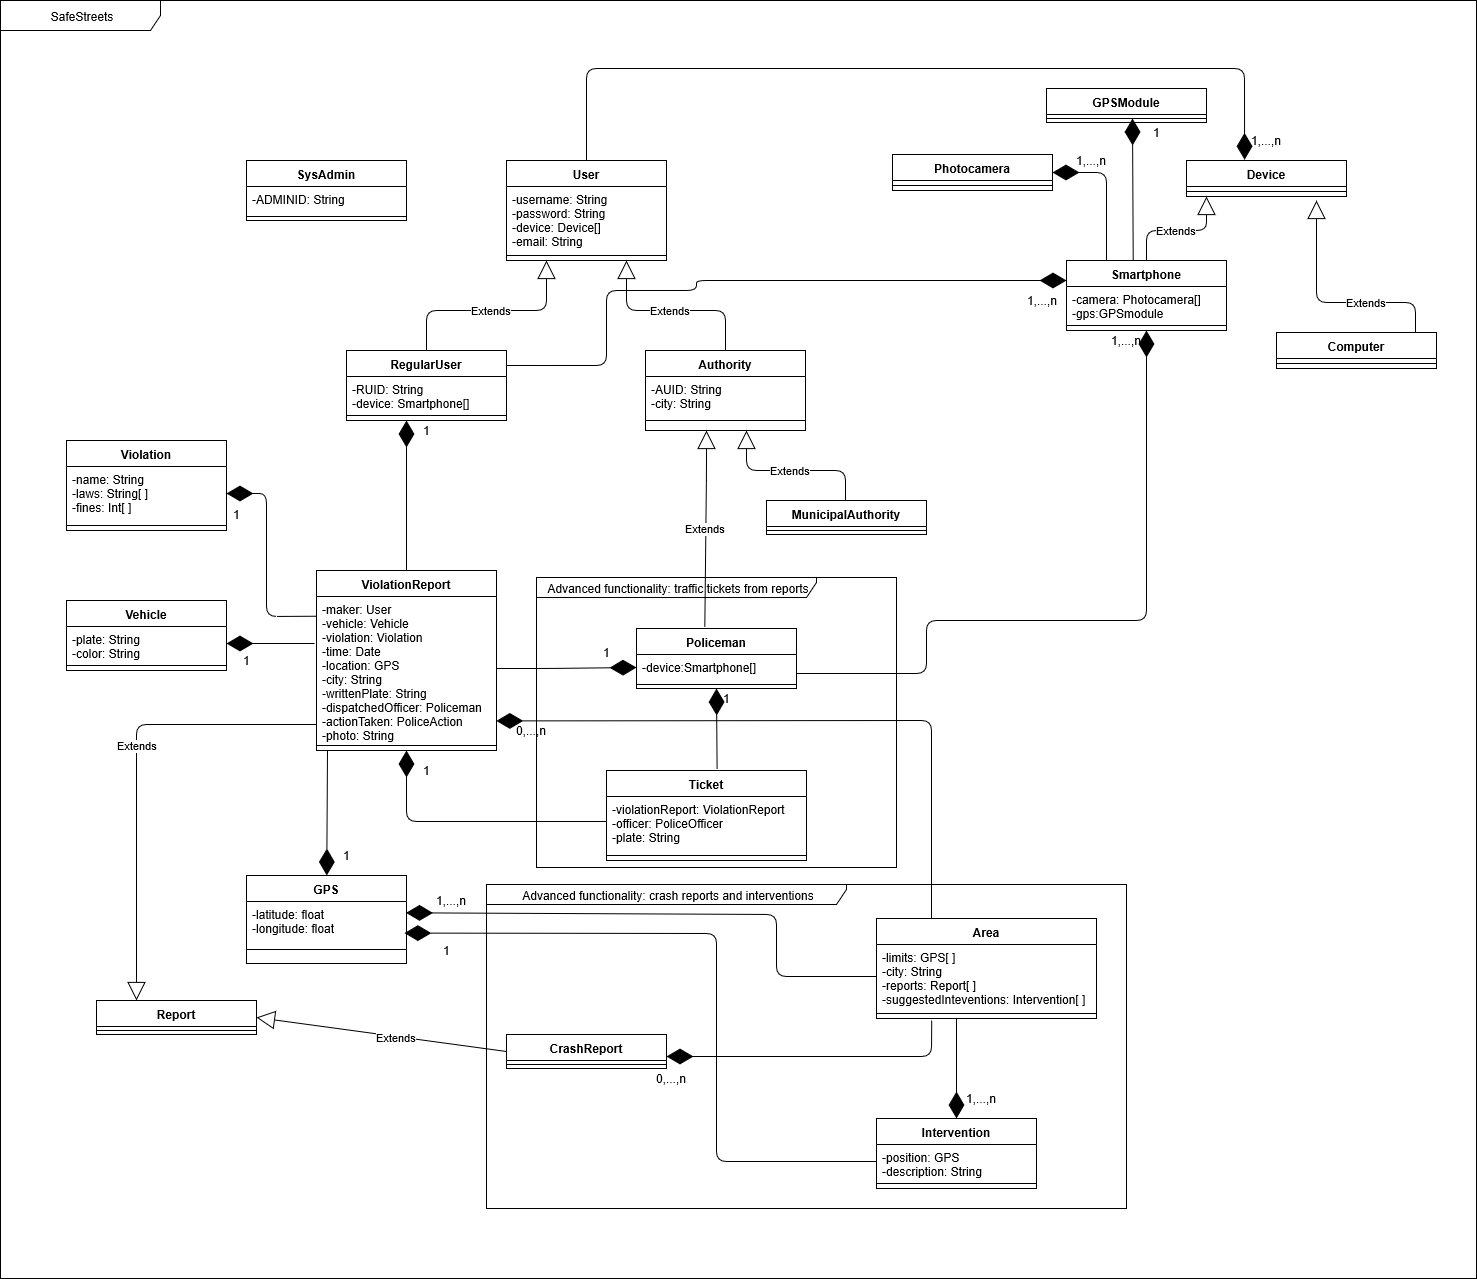
\includegraphics[width=\textwidth]{Images/ADV_class_diagram}
	\caption{Class diagram}
\end{figure}
\newpage

\begin{figure}[H]
	\centering
	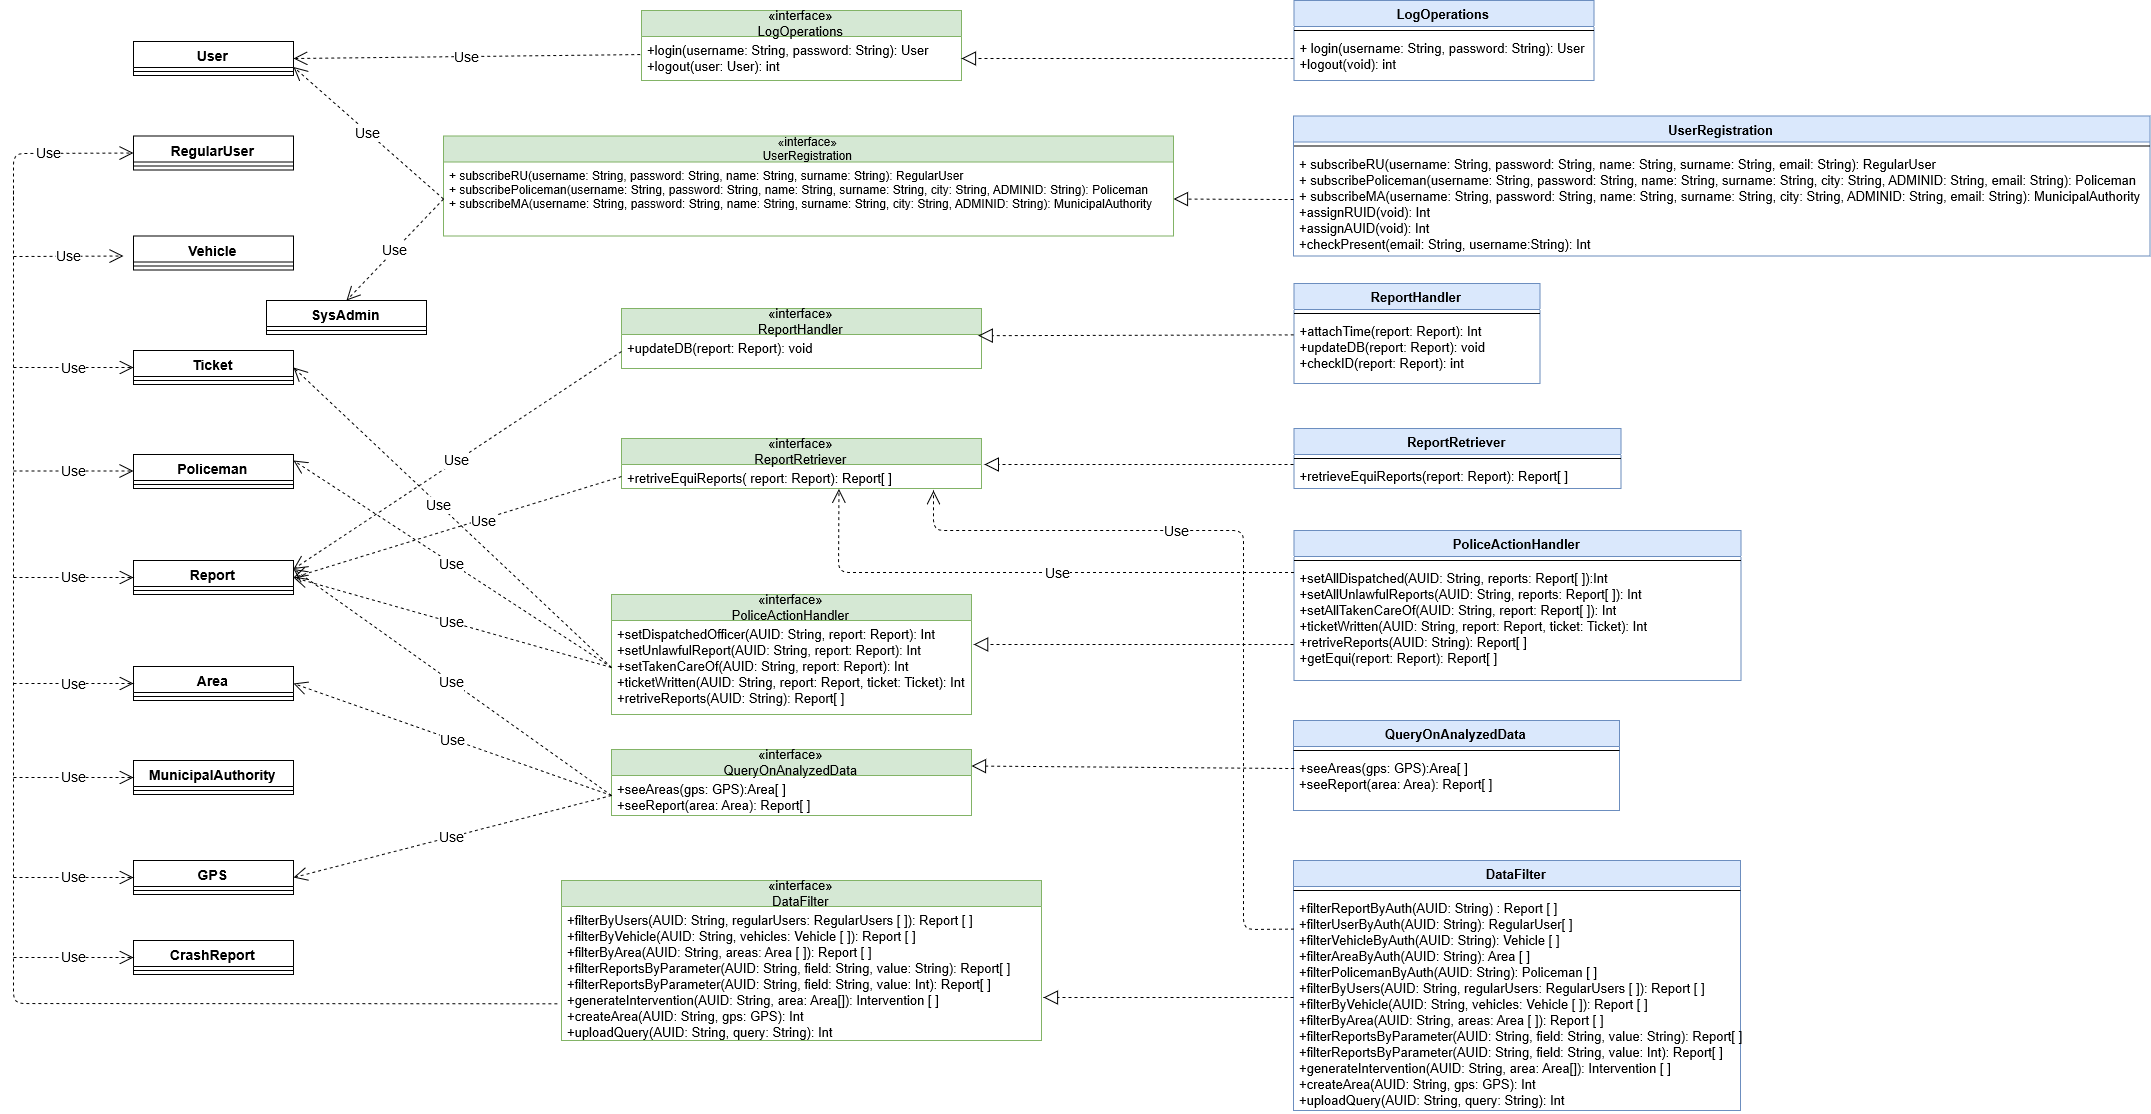
\includegraphics[angle=90, scale=0.25]{Images/component_class_relation}
	\caption{Relation between components and already specified classes}
\end{figure}
\newpage

\subsubsection{LoadBalancer}
The proprietary server approach chosen for the system may limit its scalability, since the available resources cannot be increased on the demand as in a cloud-based environment. Even though an high level of scalability is not a strict requirement for the application, we decided to insert a load balancer in order to achive better flexibility and scalability. This component should allow the system availability and funcionality even in case of heavy load, granting enough room to plan server expantions and simplifying these operations at the same time. \newline
A CISCO off-the-shelf solution is to be considered.

\subsubsection{Client}
In this section, we will give a description of the three clients functions showed in the introduction:
\begin{itemize}
	\item RegularUserClient: allows regular users to register and login to the service, to send reports about traffic violations and visualize on a map the most unsafe areas around him.
	\item PolicemenClient: allows policemen login to the service, to retrieve reports sent by the regular users (visualized in a map format) and to communicate that they are working to resolve a specific report.
	\item MunicipalAuthoritiesClient: allows municipal authorities to login to the service, to mine data about their municipality from the DataBase and to visualize violation maps, suggested interventions, advanced informations based on crossing SS data and accidents informations (if provided by the municipality).
\end{itemize}
In the following pictures we will provided more detailed informations about the three clients' components, focusing on one at a time.

\begin{figure}[h!]
	\centering
	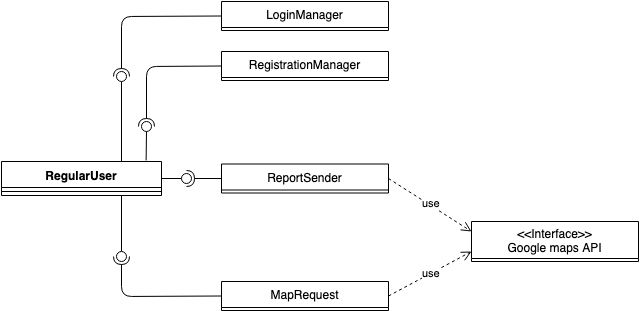
\includegraphics[scale=0.7]{Images/RegularUserClient}
	\caption{Relation between components inside regular user client}
\end{figure}
The components represented in this diagram are:
\begin{itemize}
	\item LoginManager: Allows users to send their log data to the server in order to login or logout from the system.
	\item RegistrationManager: Allows users to send  their registration data to the server in order to create a new account.
	\item ReportManager: Allows users to send a report about traffic violations, packing all the required data in a suitable format to be sent to the server. This component also uses Google maps API in order to recover informations about the area around user's geographical position.
	\item PlateRecognizer: Allows plate number recognition exploiting a classification Machine Learning algorithm. This component will be used by ReportManager during the process of building a report.
	\item MapViewer: Allows the user to visualize a geographical map from Google maps API enriched by data about unsafe areas, statistics and traffic violations coming from the server.
\end{itemize}

\begin{figure}[h!]
	\centering
	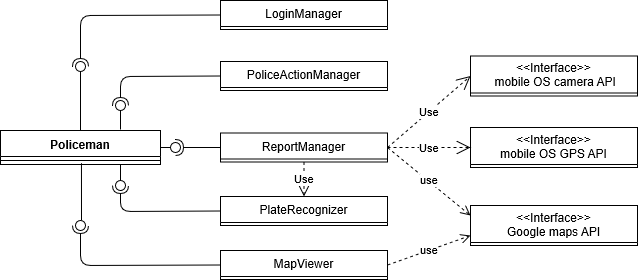
\includegraphics[scale=0.7]{Images/PolicemanClient}
	\caption{Relation between components inside policeman client}
\end{figure}

The components represented in this diagram are:
\begin{itemize}
	\item LoginManager: It has the same function as in the regular user client.
	\item ReportManager: Allows Policeman to send a traffic violation report with all the required data, packed in a correct format, to the server.
	This component also uses Google maps API in order to recover informations about the area around user's geographical position.\newline
	It's worth noting that if a policeman sends a report about a violation, he is automatically assigned to solving it.
	\item PlateRecognizer: Allows plate number recognition exploiting a classification Machine Learning algorithm. This component will be used by ReportManager during the process of building a report.
	\item MapViewer: Allows a policeman to visualize the list of the various pending reportsfor his municipality.
	The locations of theeports will be shown on a map provided through Google maps API.
	\item PoliceActionManager: Allows a policeman to signal that his intention to take care of a report. This component will send a suitable message to server which will update its data accordingly, marking the considered report as under analisys.
	
\end{itemize}
\newpage
\begin{figure}[H]
	\centering
	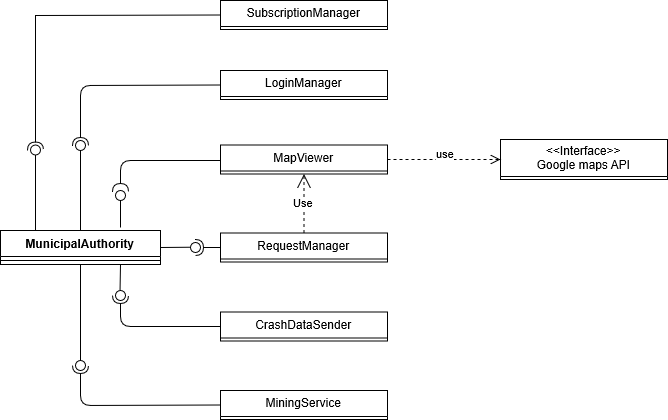
\includegraphics[scale=0.7]{Images/MunicipalAuthorityClient}
	\caption{Relation between components inside municipal authority client}
\end{figure}
The components represented in this diagram are:
\begin{itemize}
	\item LoginManager: It has the same function as in the regular user client.
	\item RequestManager: Allows the municipality to request data about Reports (solved or not) from the server. This componet uses MapViewer in order to provide violation data in a map format.
	\item MapViewer: Allows the visualization of the mined data in a map format. This component exploit Google Maps API to provide a representation of the local map.
	\item CrashDataSender: Allows the municipal authority to send Data about car crashes around the municipality to the server in order to be crossed with data already collected.
	\item MiningService: Provides an interface to simplify the acess of collected data to the municipality.
\end{itemize}

\newpage
\subsection{Deployment view}

\begin{figure}[h!]
	\centering
	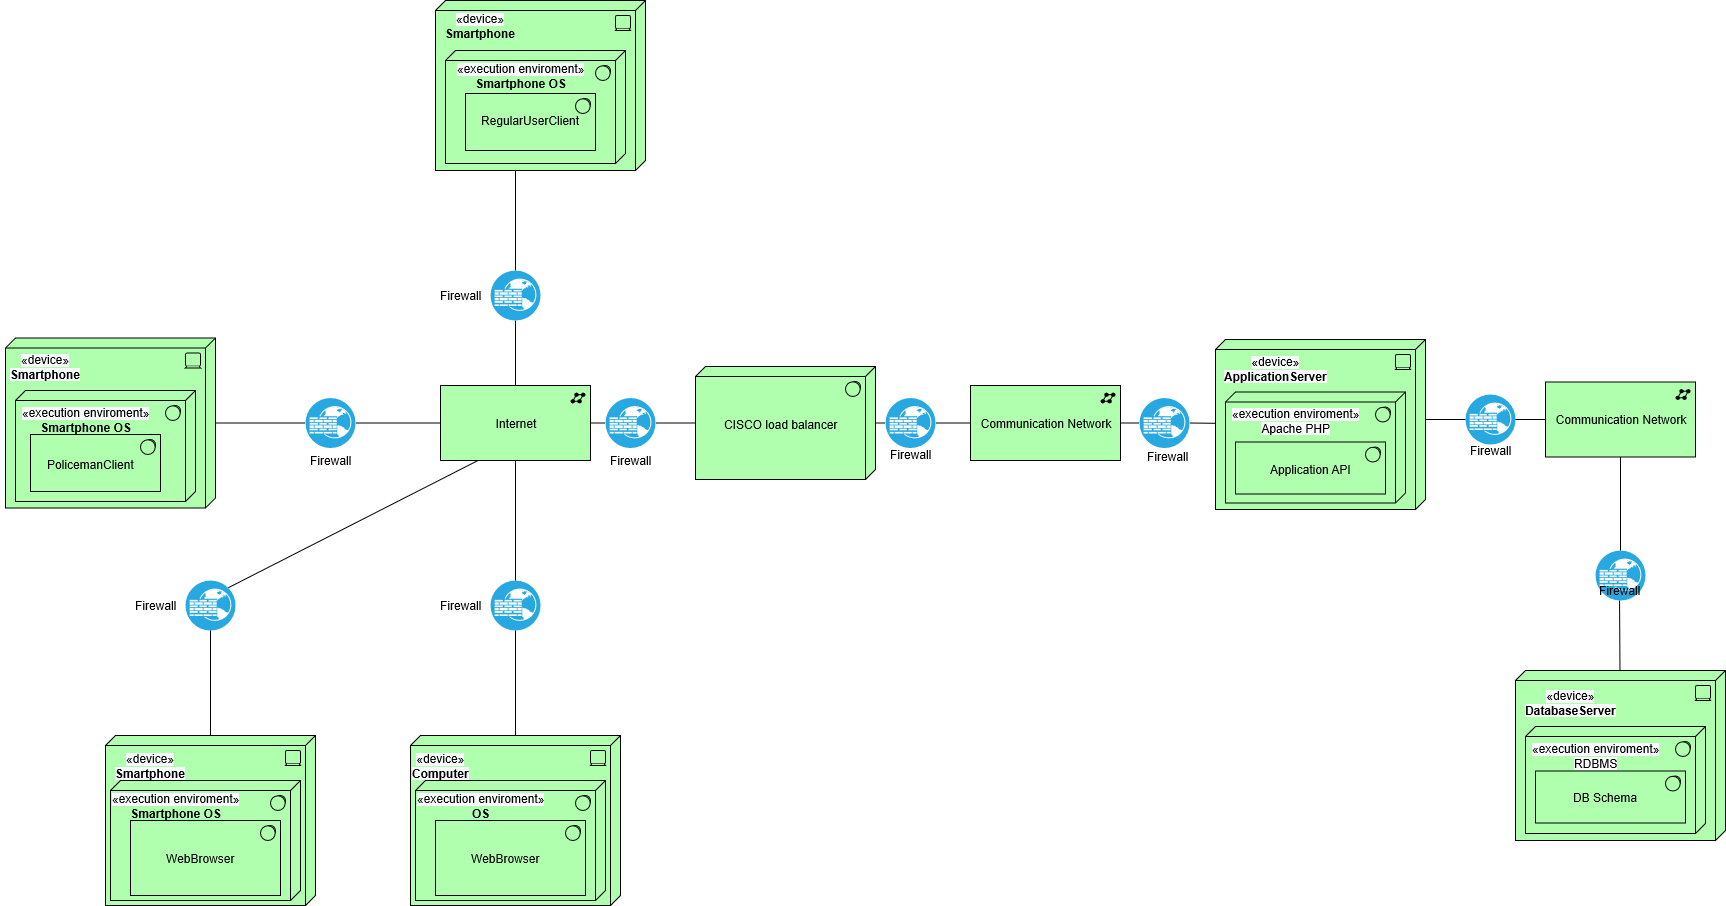
\includegraphics[width=\textwidth]{Images/physical_view}
	\caption{Physical view}
\end{figure}

The image above shows the system's architecture from a physical standpoint.
Components:
\begin{itemize}
\item Smartphone: Device used by both RegularUser and Policeman users type to interact with the application. Two different clients will be developed: one for regular users, that will allow them to look at already analyzed data and submit reports, and a different one for policemen, that will allow the officers make reports (upon which they will take actions right away) and take actions on reports
\item Computer: device used by MunicipalAuthorities users. They will interact with the application via a web page, that will allow them to interact in various ways with the Reports submitted by the other users.
\item Load Balancer: CISCO off-the-shelf load balancer
\item Application server: this server contains the application logic and will interact with the different clients in a client-server way.
\item DatabaseServer: this server contains the actual data, both about the registered users and related to the user submitted reports, the actions taken by the police and the results of the data mining operations done by municipal authorities
\end{itemize}
Please note that Google servers have not been included, since those servers will not be involved in the system deployment
\newpage

\subsection{Runtime view}
In this section the main functionalities of the system are analyzed through the use of sequence diagrams. The participants involved in the diagrams are either system componets (from client and server side) or external services APIs (e.g. Google Maps API) previuosly specified in this document.\newline
A colour schema has been used in order to increase diagram clarity: Client components are represented with light blue labels; Server components with yellow labels; third party API with green labels.

\medskip

\begin{figure}[H]
	\centering
	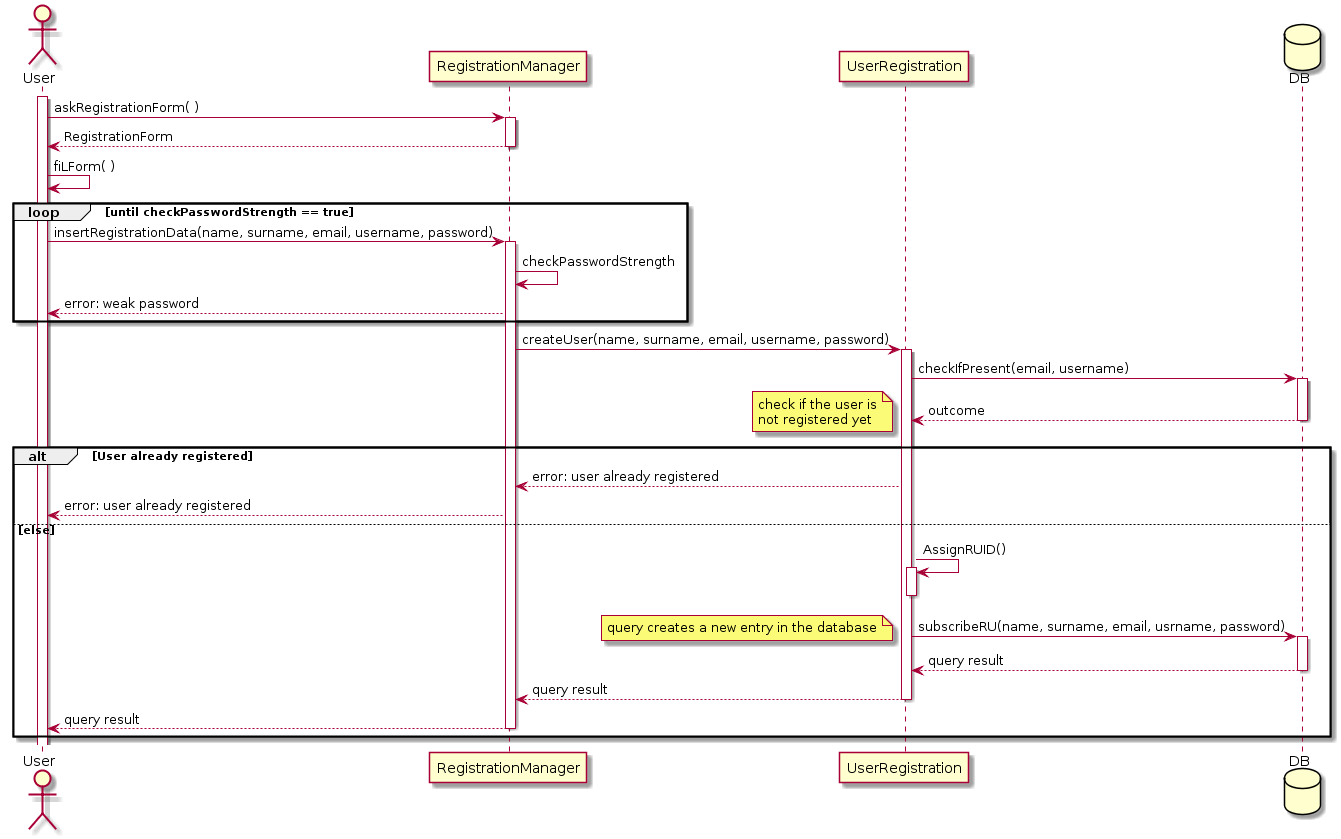
\includegraphics[width=\textwidth]{Images/seqDiag_userReg}
	\caption{User registration process}
\end{figure}
	\newpage

\begin{figure}[H]
	\centering
	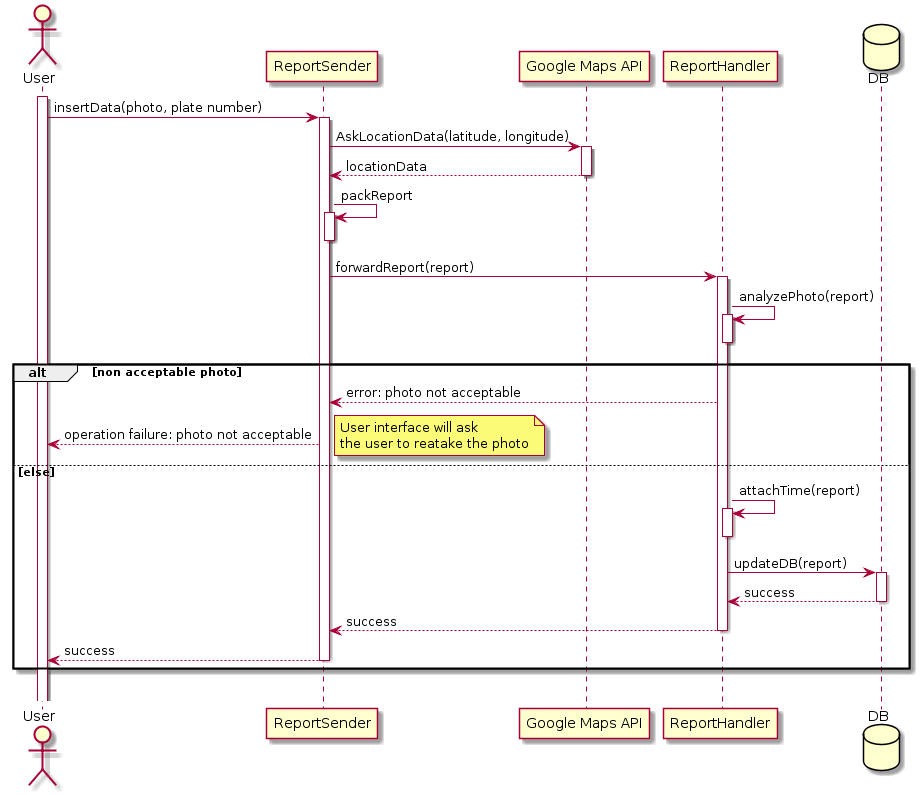
\includegraphics[width=\textwidth]{Images/seqDiag_ReportSignal}
	\caption{Report signaling procedure}
\end{figure}
	\newpage	
	
\begin{figure}[H]
	\centering
	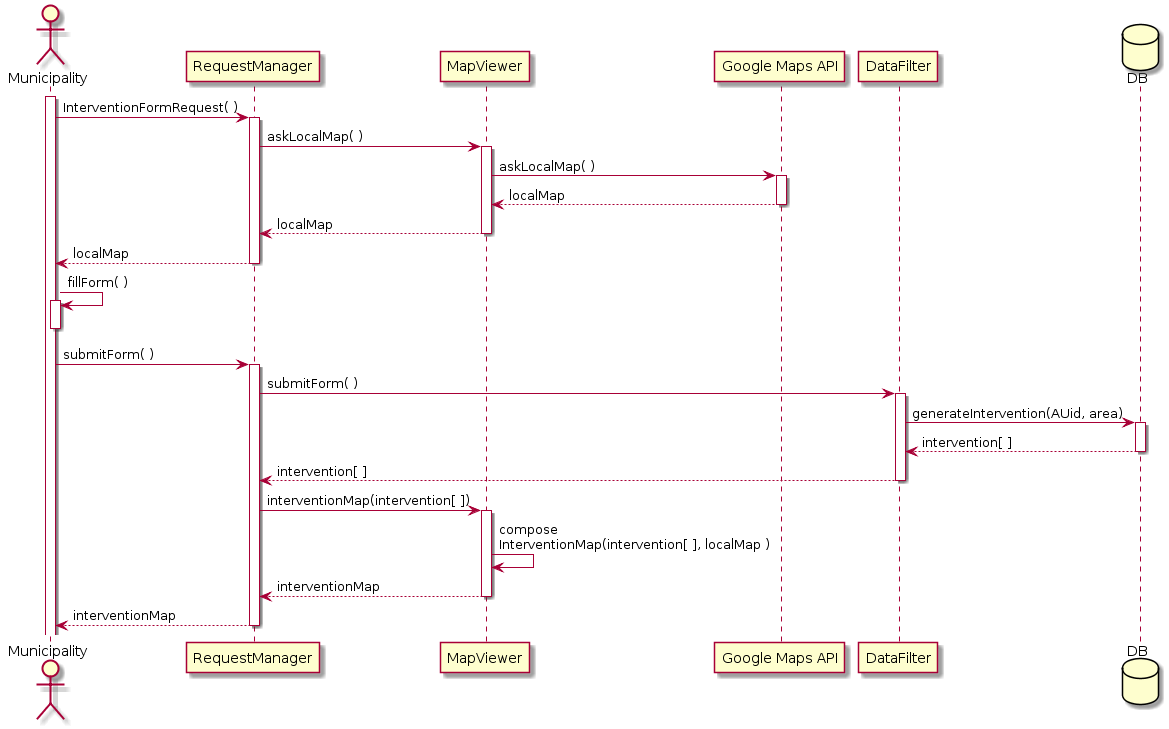
\includegraphics[width=\textwidth]{Images/seqDiag_Interventions}
	\caption{Municipality query for possible intervention in its metropolitan area}
\end{figure}
	\newpage

\begin{figure}[H]
	\centering
	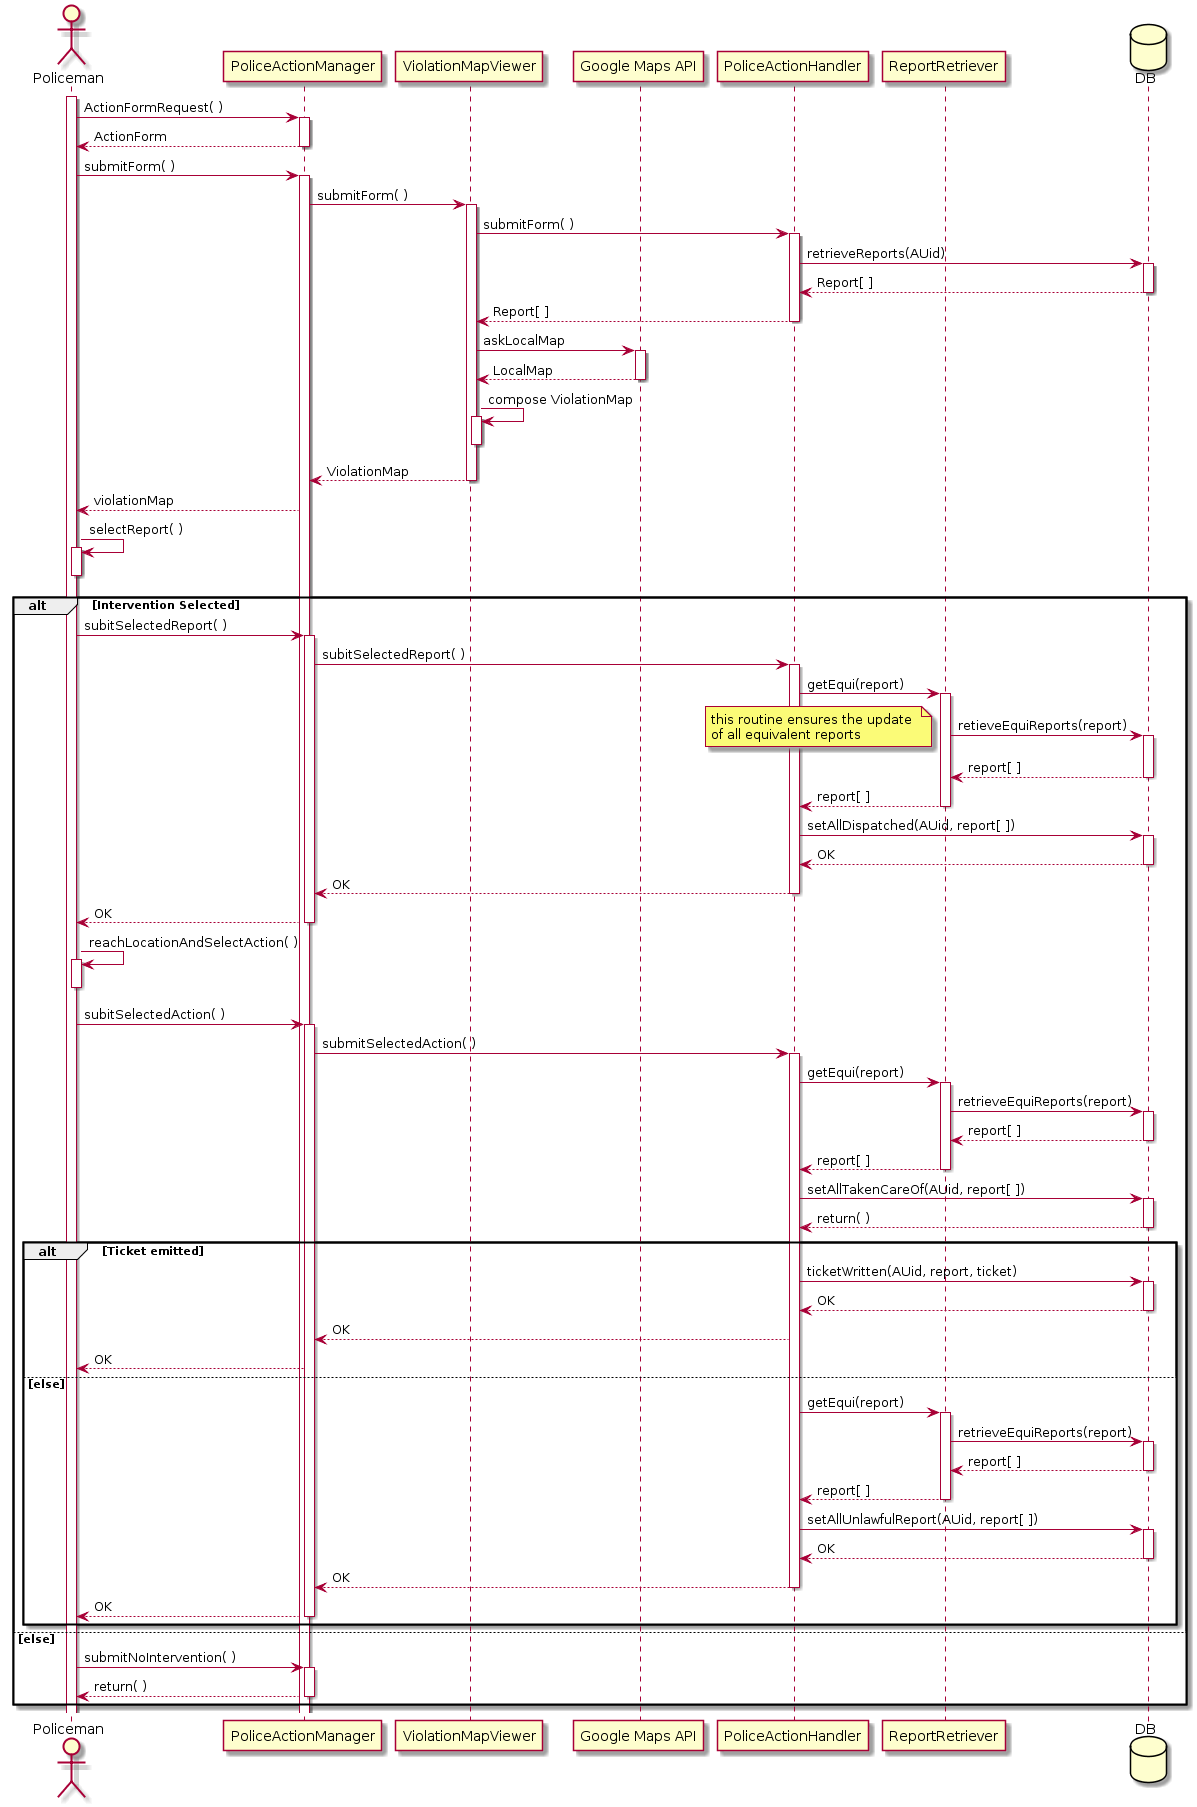
\includegraphics[width=\textwidth]{Images/seqDiag_PolicemanAct}
	\caption{Policeman takes care of a signaled report}
\end{figure}


\subsection{Interfaces}
\begin{figure}[H]
	\centering
	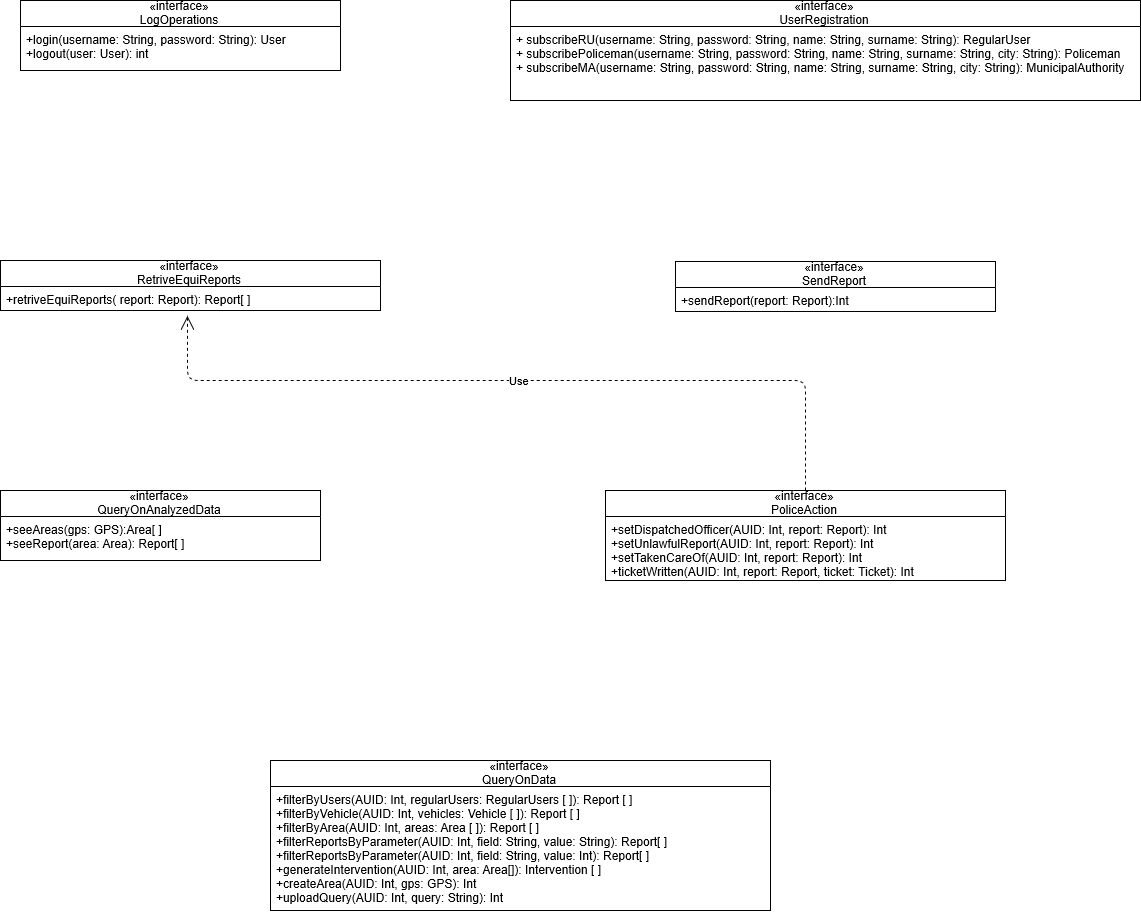
\includegraphics[width=\textwidth]{Images/interface_diagram}
	\caption{Components' interfaces}
\end{figure}
Other than the relation between PoliceActionHandler, DataFilter and ReportRetriever, already explained in section 2.2, it is worth noting that the interfaces don't actually expose all the methods of the objects that implement them. This choice was made in order to hide the methods that will be called only from inside the object in which they are defined.
\newpage 

\subsection{Architectural and implementative styles and patterns}

\subsubsection{Architectural styles}
\begin{itemize}
	\item Client-server: given the nature of the application, a distibuted system in which data submitted by some users has to be accessible by other users, the figure of a mediator becomes necessary. Therefore a client-server architecture seems to be a good solution. Another alternative could have been a cloud computing architecture (SaaS, flex tenacity approach), but we opted for a client-server architecture since the workload and scalability issues would not be big enough to justify the increased costs.
	\item Thin client: in the aformentioned client-server architecture, the role of the server is more than just a message manager. As a matter of fact, the server also takes care of the application logic, allowing a light client with limited functionalities.
	\item Three tiers architecture: given the client-server with thin client architecture described, the most natural solution is a three tier architecture in which the presentation layer is on the client, the application layer on the application server and the data layer on the database server. 
\end{itemize}

\subsubsection{Design patterns}
\begin{itemize}
	\item Model-view-controller: given the three-tiers and thin client architecture, using a MVC design pattern is quite easy: the model will be represented by the database server, the control by the application server and the view will be managed by the client. \newline
	The development of a different view for each type of user will be necessary, considering the different privileges and functions offered. Thus, in this section of the system modularity of the application will be central: sharing of common modules will simplify the development. 
	\item Facade: used to hide components complexity; useful to isolate functionality, improve portability and maintainability. In particular this will ease clients development since the 3 client proposed share many modules.
	\item Oberserver-Oberservable: considering the message-driven architecture of the system, this pattern can be used to model components comunication.
	\item Factory: used in clients to create reports and in general messages and requests.
\end{itemize}

\subsection{Other design choiches}
This sections explores many meaningfull design decisions that deserve further specification.

\begin{itemize}
	\item Plate Recognition Procedure: Here we present a brief description of the steps of the photo analysis routine, contextualizing it in the report signaling flow.
	\begin{itemize}
		\item Entry conditions: during a standard report procedure (the whole procedure is handled by ReportManager component), the user is propted to take a photo of the violation.
		\item  Procedure steps:
	\begin{enumerate}
		\item Image acquisition: the ReportManager client component, interfacing with OS camera API, presents the user a in-app camera interface. The user takes a photo of the violation.
		\item Image cropping: the user is asked to crop the image, in order to obtain a picture representing only the plate involved in the violation. This step is necessary to avoid possibile problems with pictures including more than a plate. In addiction, the image cropping reduces a lot the computation resources needed for a plate recognition algorithm.\\
		The GUI has to offer a basic tool for image cropping, such as a floating selection rectangle.
		\item Plate number recognition:  the client runs locally an image recognition algorithm. \\
		A classification machine learning algorithm has been chosen for this task. Given the small set of possible simbols involved and the standardization of this simbols, the neural net required will be easly developed and trained. Moreover, virtually every smartphone can easly run a net of this kind. Thus, we opted to integrate the net into a client component, the PlateRecognizer.\\
		Note that the performance consideration presented apply exclusively to an image representing only a plate: so the image cropping step is vital.
	\end{enumerate}
	\item Output conditions: the recognition algorithm return a plate number that will be compared to the number manually inserted by the user.
	\end{itemize}
	\item Security concerns: as expressed in the RASD, there are various measures needed in order to obtain a good level of security:
	\begin{itemize}
		\item Filtering and escaping registartion requests of all kinds of user profiles and RegularUser submitted reports (Policeman submitted ones and MunicipalAuthority queries are considered trustwothy) in order to avoid code injections
		\item Escaping and filtering login fields in order to avoid code injections
		\item All communication must happen over a secure channel (HTTPS)
		\item An anti cross site request forgery token is needed, in particular for Municipal Authority web interface
	\end{itemize}
	\item Database: for this application a relational database has been chosen, since involving any other kind of solution would be a waste of resources for no sensible inprovement on the system
	\item All exchanged data are in xml format (all the photos are hashed via base 64 and embedded in the document)
\end{itemize}